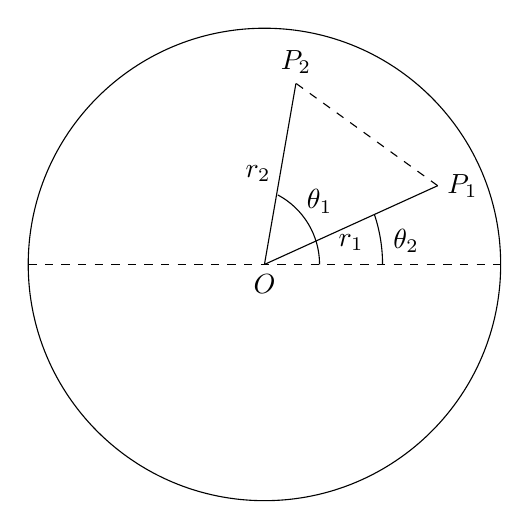
\begin{tikzpicture}
    \coordinate [label=above:$P_2$]   (P2) at (0.4,2.3);
    \coordinate [label=right:$P_1$]   (P1) at (2.2,1  );
    \coordinate (A) at (-3,0);
    \coordinate (B) at ( 3,0);
    \coordinate (M) at (1.5,0);
    \coordinate (N) at (0.7,0);
    \coordinate (K) at (0.7,0.8);
    \coordinate (L) at (1.8,0.3);

    \coordinate [label=below:$O$]            (O) at ( 0,0);

    \draw[dashed] (A)  -- (B);
    \draw[dashed] (P1) -- (P2);

    \draw (O) -- node[midway,below]{$r_1$} (P1);
    \draw (O) -- node[midway,left] {$r_2$} (P2);

    % Triangles
    %\draw (P) -- node[midway,below]{$d$} (O) -- (B) -- cycle;
    %\draw (O) -- node[midway,above,sloped]{$a$} (B);
    %\draw[dashed] (O) -- (A);

    % Circle
    \draw (0,0) circle (3cm);

    % Arc for Angle
    \draw (M) arc (0:18.5:2);
    \draw (N) arc (0:62:1);

    \node at (K) {$\theta_1$};
    \node at (L) {$\theta_2$};
\end{tikzpicture}
